\documentclass[../main.tex]{subfiles}
\begin{document}

\subsection{GANs proof of concept}
To test the adversarial setting versus a more traditional loss: \gls{mse}
(equation \ref{eq:mse}),
a ``toy example'' is carried out\footnotemark: train a generator
model to fit a normal distribution with mean 0 and variance 1 ($p_{data}$).
\footnotetext{Code available at \url{https://github.com/gio8tisu/GAN-PoC}}

The generator samples a vector of length 5
from a uniform ditribution (range -0.5-0.5) ($p_z$) and passes
it through 3 fully connected layers\footnote{A fully connected layer outputs
the matrix product between its input and a weights matrix and adds a bias vector,
a node/neuron represents a row in the weight matrix plus the corresponding
element in the bias vector: $\tensor{y} = \tensor{W}\tensor{x} + \tensor{b}$, where
$\tensor{x}$ is the input represented as a column vector.}
with LeakyReLU activation function and 5 units on each layer except for the
final layer which only has 1 unit (it outputs a scalar) and no activation
function (represented in figure \ref{fig:gan-poc-generator}).

\begin{figure}[h]
\centering
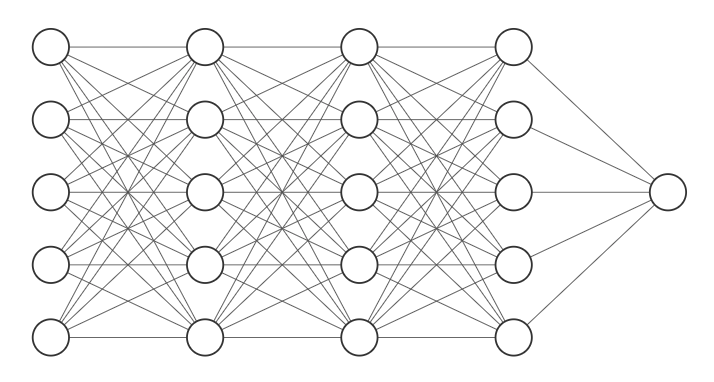
\includegraphics[width=0.4\linewidth]{gan-poc-generator}
\caption{Generator architecture used for both the \gls{mse} and \gls{gans}
setting}
\label{fig:gan-poc-generator}
\end{figure}

The target data comes from a sample of 100,000 i.i.d normal random
variables.  The models are trained for 100 epochs with a batch size of 100
using the Adam optimization algorithm presented in section \ref{sec:optimizers}
with a learning rate of $5 \times 10^{-4}$ and default momentum values.

The results are compared by computing the Kolmogorov-Smirnov test of
normality\footnote{The test statistic provides a measurement of the divergence
of your sample distribution from the normal distribution.
The higher the value of D, the less probable  the data is normally distributed.
The p-value quantifies this probability, with a low probability indicating that
the sample diverges from a normal distribution to an extent unlikely to arise
merely by chance.  It is computed
using the \url{https://www.socscistatistics.com/tests/kolmogorov} online tool.}.

\subsubsection{Results for \gls{mse} loss}
As to be expected, the \gls{ann} simply ignores the source of randomness
(set first layer's weights close to zero) and produces an almost deterministic
output close to the distribution's expected value: this is in fact the optimal
solution for the \gls{mse} objective function.

\begin{equation}\label{eq:mse}
L(G_{\theta}(\tensor{x}), \tensor{y}) =
\left\| \tensor{y} - G_{\theta}(\tensor{x}) \right\|_2^2
\end{equation}

Example of generated samples:
\verb|-0.05046 -0.05155 -0.05082 -0.05044 ...|

The value of the K-S test statistic for 300 samples generated by this model is 0.1023.
The p-value is 0.01819. This provides good evidence that the data is not
normally distributed.

\subsubsection{Results for adversarial loss}
Rather than training $G$ to minimize $\log (1 - D(G(\tensor{z})))$,
$G$ is trained to maximize $\log D(G(\tensor{z}))$.
This is a common practice as equation
\eqref{eq:generator} may not provide sufficient gradient for $G$ to learn well
early in training. It follows the same principle: try to fool the disctiminator.

\begin{equation}
L(G_{\theta}(\tensor{x}), \tensor{y}) = - \log D(G(\tensor{z}))
\end{equation}

The discriminator network is composed of 3 hidden layers with LeakyReLU as well,
with a sigmoid activation function in the output layer.

\begin{figure}[h]
\centering
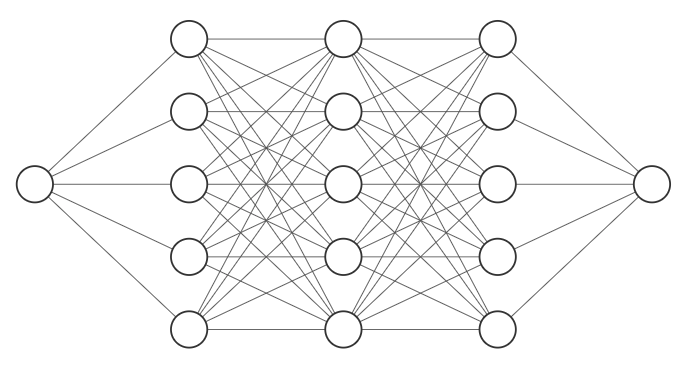
\includegraphics[width=0.4\linewidth]{gan-poc-discriminator}
\caption{Discriminator architecture}
\label{fig:fig:gan-poc-generator}
\end{figure}

In the case of the generator network traned in an adversarial manner,
it produces samples with variability that are close to normally disributed
(see figure \ref{fig:gan-poc} for a visual comparison with a true normal
distribution).

The value of the K-S test statistic for 300 samples generated by this model is 0.03383.
The p-value is 0.87045. This provides good evidence that the data does
not differ significantly from that which is normally distributed.

This model clearly beats the \gls{mse} one on producing realistic and varied
samples, but the training was much more unstable and the problem of mode
collapse was encountered. Several training iterations with different
hyperparameters (like number of layers, activation functions, learning rate,...)
were necessary.

\begin{figure}[h]
\centering
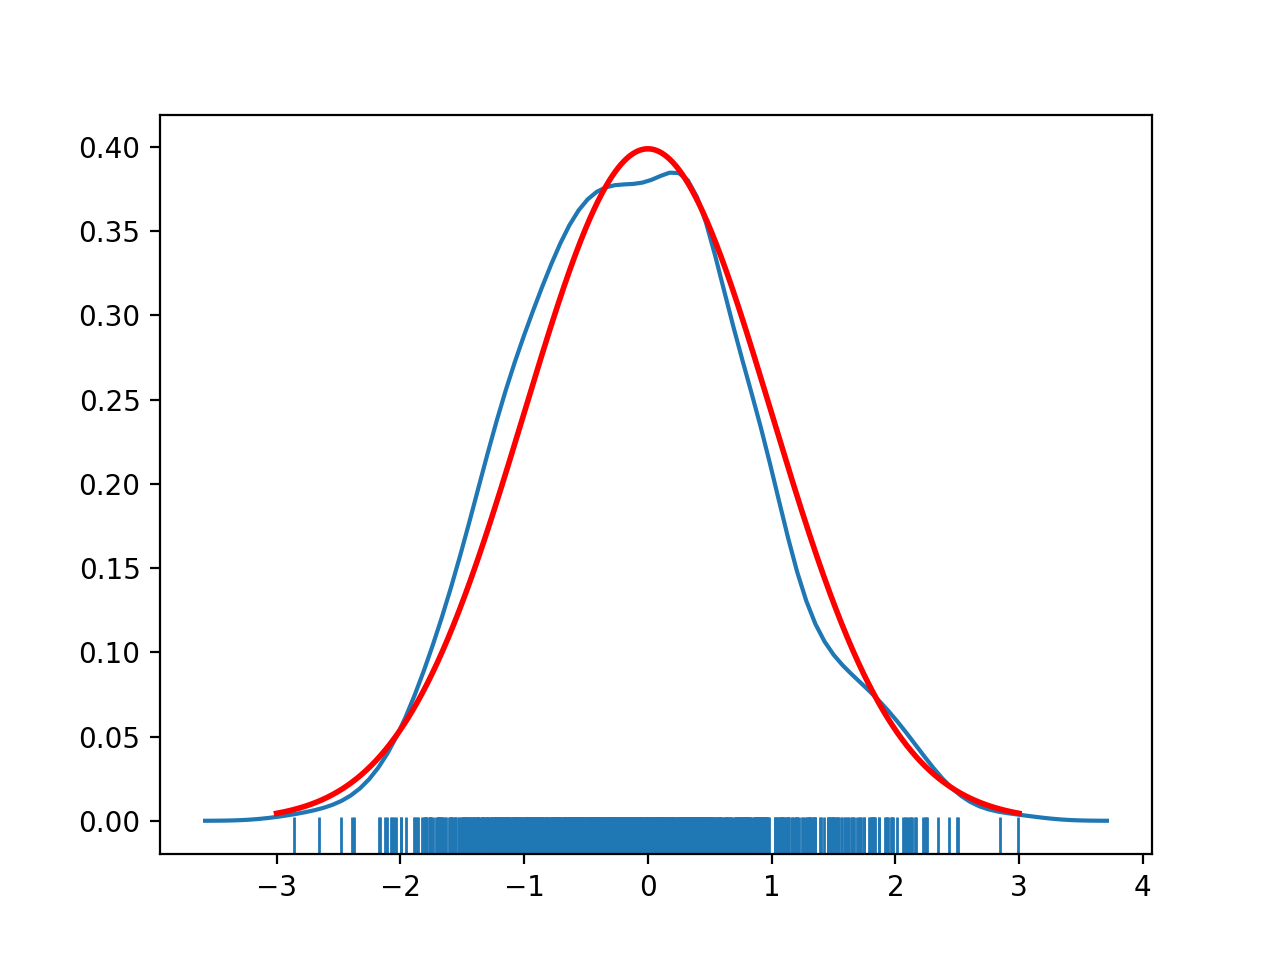
\includegraphics[width=0.5\linewidth]{gan-poc}
\caption{In blue a plot of the kernel density estimation using 1000
samples from the generator trained through the \gls{gans} framework.
In red the probability density function of a normal random variable.}
\label{fig:gan-poc}
\end{figure}

\subsection{Despeckling network}

The loss function used to define the objetive function the model
will learn on is the \gls{mse} between \gls{fcm} $256 \times 256$ crops and
the artificially contaminated  version of it.
\begin{subequations}
\begin{equation}
L(f_{\theta}(\tensor{x}_{noisy}), \tensor{x}_{clean})
= \left\| \tensor{x}_{clean} - f_{\theta}(\tensor{x}_{noisy}) \right\|_2^2
\end{equation}
\begin{equation}\label{eq:noisy}
\tensor{x}_{noisy} = \tensor{x}_{clean} \odot \tensor{s}
\end{equation}
\end{subequations}
Where $\tensor{s}$ is a realization of the speckle noise random variable model.

\subsubsection{Model selection}
As explained in section \ref{sec:despeckling-network},
three different network architectures
are implemented. To evaluate the model performance, a comparison of the \gls{ssim}
(\cite{Wang2004}) between noisy and clean (denoted $SSIM_{input}$);
and denoised and clean (denoted $SSIM_{output}$) is used.
Due to the lack of information about the confocal microcope used,
the experiments are done with 2 different values $\{1, 5\}$ for the parameter
$L$ of the noise model \eqref{eq:gamma-distribution}.

The division skip-connection model is discarded early in the process because
it fails to find any solution close to the desired.

\begin{figure}[h]
\centering
\begin{subfigure}{.5\textwidth}
  \centering
  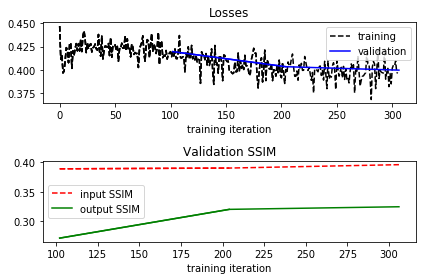
\includegraphics[width=.8\linewidth]{divide-learning-curve}
  \caption{Learning curve or the division skip-connection model.
  $SSIM_{input}$ is greater than $SSIM_{output}$ throughout the trianing
  process}
  \label{fig:divide-learning-curve}
\end{subfigure}%
\begin{subfigure}{.5\textwidth}
  \centering
  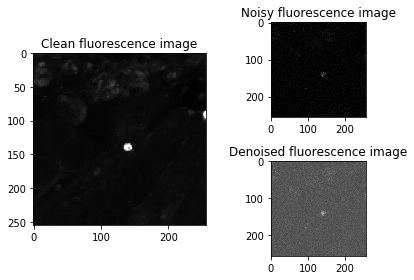
\includegraphics[width=.8\linewidth]{divide-denoised}
  \caption{Example of denoised \gls{fcm}}
  \label{fig:divide-denoised}
\end{subfigure}
\caption{The division skip-connection model fails to converge.}
\label{fig:hallucination}
\end{figure}

In table \ref{tab:despeckling} the mean SSIM values on the validation set
for each of the final models are shown. The training process is done during
20 epochs using the Adam optimizer with a learning rate of $10^{-3}$ and a
batch size of 32 samples.

\begin{table}
\centering
\begin{tabular}{*5c}
\toprule
Model & $M$ & $K$ & $N$ & mean $SSIM_{output}$ \\
\midrule
Multiply ($L = 1$) & 3 & 32 & 5 & 0.877 \\
Multiply ($L = 1$) & 5 & 64 & 5 & 0.728 \\
Multiply ($L = 5$) & 5 & 64 & 5 & 0.947 \\
Log-Add ($L = 1$) & 3 & 32 & 5 & 0.960 \\
Log-Add ($L = 1$) & 5 & 64 & 5 & 0.806 \\
Log-Add ($L = 5$) & 5 & 64 & 5 & 0.965 \\
\bottomrule
\end{tabular}
\caption{Models comparison with different number of layers $M$, number
of filters $K$ and filter size $N$. The validation set mean $SSIM_{input}$
is 0.414 for $L=1$ and 0.723 for $L=5$}
\label{tab:despeckling}
\end{table}

\subsection{Staining network}
\subsubsection{Baseline}
The baseline presented in \ref{sec:stain-baseline} is trained using the
Adam optimizer
with a batch size of 8, learning rate of $5 \times 10^{-4}$, momentums of
0.5 and 0.999 for $\beta_1$ and $\beta_2$ respectively. This hyperparameter
values provide the best looking results, as with other parameters the training
quickly destabilizes.

To provide an initialization closer to the optimal one, the weights are
initializated with the weights defined by \cite{Gareau2009} transformation.

The final results are very similar to the ones of the initial state,
(see figure \ref{fig:stain-baseline})
so the model makes no real progress to make a better looking stain version.

\begin{figure}
\centering
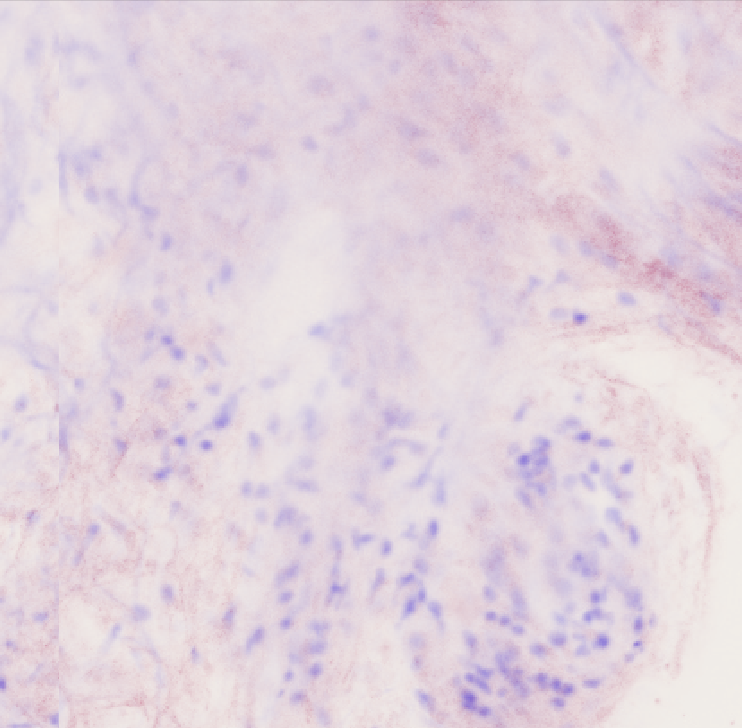
\includegraphics[width=0.4\linewidth]{stain-baseline}
\caption{Example of a crop stained by the baseline model}
\label{fig:stain-baseline}
\end{figure}

\subsubsection{Advanced \gls{dnn}}

\begin{figure}
\centering
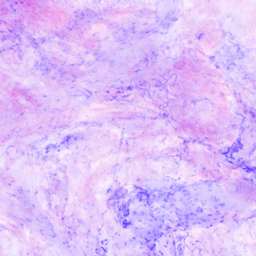
\includegraphics[width=0.4\linewidth]{1038_real_A}
\caption{}
\label{}
\end{figure}

The two architectures are trained using the hyperparameters described
in table \ref{tab:hyperparameters} 
for tand instead of optimizing the
original GAN objective
the so-called LSGAN ---use the L2 distance instead of the cross-entropy---
is used which is empirically shown to provide a more
stable training (\cite{lsgan}).

In theory the UNet-like model shoud mantain the structure and be less prone
to ``hallucinate'', in practice this generally holds but still some structures
are made up by the model; the residual model on the other hand sometimes
eliminates nuclei present in the source image. Both cases can be seen in figure
\ref{fig:resnet-unet}.

The mean value of the \gls{lbp} histogram distance for the validation
set is 0.0332 for the residual model and 0.0183 for the unet.

\begin{table}
\centering
\begin{tabular}{cc}
\toprule
hyperparameter & value \\
\midrule
$\lambda_{cycle}$ & 10 \\
$\lambda_{identity}$ & 5 \\
learning rate & $2 \time 10^{-4}$ \\
$\beta_1$ & 0.5 \\
$\beta_2$ & 0.9 \\
epochs & 200 \\
\#layers $D$ & 3 \\
residual blocks (residual model) & 9 \\
\# down-sampling layers (UNet model) & 7 \\
\bottomrule
\end{tabular}
\caption{Table of hyperparameters used in staining network}
\label{tab:hyperparameters}
\end{table}

\begin{figure}[h]
\centering
\begin{subfigure}{.5\textwidth}
  \centering
  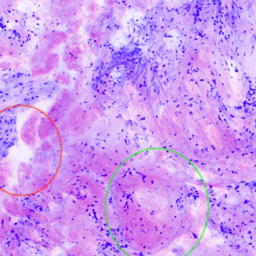
\includegraphics[width=.8\linewidth]{104_real_A}
  \caption{Real}
  \label{fig:real-example}
\end{subfigure}
\begin{subfigure}{.5\textwidth}
  \centering
  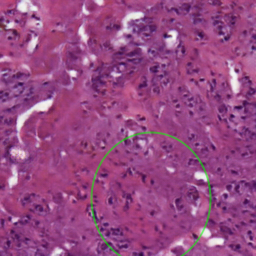
\includegraphics[width=.8\linewidth]{104_fake_B-resnet}
  \caption{Residual network}
  \label{fig:resnet-example}
\end{subfigure}%
\begin{subfigure}{.5\textwidth}
  \centering
  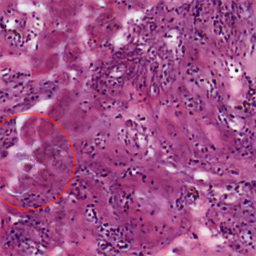
\includegraphics[width=.8\linewidth]{104_fake_B-unet}
  \caption{UNet-like}
  \label{fig:unet-example}
\end{subfigure}
\caption{(a) is the models' input, the second row show the outputs for the
respective models. On (b) some nuclei that are in the input have been
erased by the network ---marked in green---. On (c) some structures are
generated that are not present in the input ---marked in red---.}
\label{fig:resnet-unet}
\end{figure}

\subsection{Inference method}
The 2 of th inference methods described in section \ref{sec:inference} are
compared by
computing the mean chi-squared distance of $512 \times 512$ patches 
in 7 large slides,
i.e.: from a \gls{cm} large mosaic, the digitally stained
version by \cite{Gareau2009} is computed (DSCM), the selected inference method
is used to produce the \gls{he} version using the U-Net model and the DSCM
as input, then these are divided with a grid of $512 \times 512$ cells and the
\gls{lbp} histogram is computed on each cell, once the histograms are computed
the chi-squared distance is used to measure how similar each cell is.

The plot in figure \ref{fig:inference-comparison} shows how the method using
50\% overlap and the weight metrix defined in \ref{} has a lower distribution
of the metric for 7 different samples.

\begin{figure}
\centering
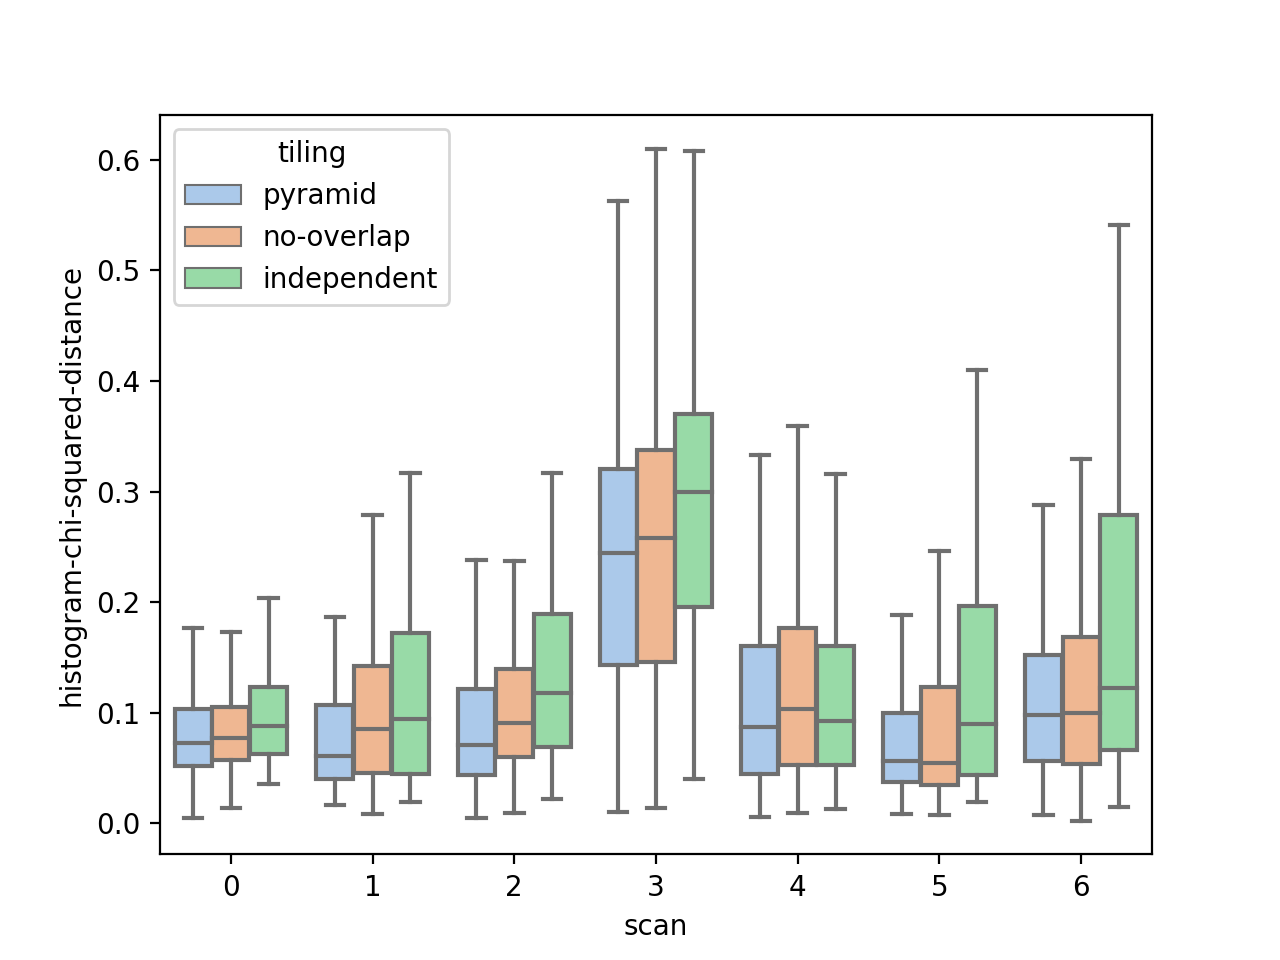
\includegraphics[width=0.6\linewidth]{inference-boxplot}
\caption{Independent tiling refers to inference made tile-by-tile with no overlap
whatsoever. No-overlap refers to the technique where the inputs have overlap but
the output is cropped so that they do not overlap. Pyramid is the WSI inference
technique from \cite{Bel2019}.}
\label{fig:inference-comparison}
\end{figure}

% \subsubsection{Histology Professionals Validation}
% \lipsum[3]

\end{document}
